\documentclass[final,5p,times,twocolumn]{elsarticle}
\usepackage{amssymb}
\usepackage{amsmath}
\usepackage{subcaption} 
\usepackage{tikz}
\usepackage{tikz-3dplot}
\usetikzlibrary{positioning, shapes.geometric, decorations.pathreplacing, calc}
\usepackage{booktabs}
\usepackage{multirow}
\journal{Measurement}

\begin{document}
\begin{frontmatter}

\title{Voiceprint Diagnosis Method for Transformer Faults Based on Mel-GADF-PCNN and Improved Physics-Informed Neural Networks} 

%\author{Chen Yang}
%\author{Zonglong Bai\corref{cor1}}
%\cortext[cor1]{corresponding author}
%\author{Chenggang Liu}
%\author{Junyan Zhang}
%\author{Yihe Guo}

%\affiliation{organization={North China Electric Power University},
%            city={Baoding},
%            postcode={071003}, 
%            country={China}}
            

\begin{abstract}
Power transformers play a vital role in ensuring power system reliability, making accurate fault diagnosis essential for operational stability. This study presents an multimodal diagnostic approach that overcomes the limitations of conventional single-spectrogram analysis. The proposed method first converts transformer acoustic signals into fused representations by combining mel spectrograms with gramian angular difference fields. A pulse-coupled neural network then enhances discriminative features while suppressing noise. Finally, the optimized AlexNet-SE architecture, developed within a physics-informed neural network framework, achieves robust fault classification. Experimental results demonstrate superior accuracy of 98.48\%, highlighting the method's practical utility for real-world grid maintenance.
\end{abstract}

\begin{keyword}Transformer faults diagnosis \sep Mel spectrograms \sep Gramian angular field \sep Feature fusion \sep Pulse coupled neural network \sep Physics-informed neural network.
\end{keyword}

\end{frontmatter}


\section{Introduction}
Power transformers are indispensable in modern power systems. Continuous monitoring and analysis of their operational status are critical to maintaining grid safety, reliability, and stability \cite{HE2026119781,10492658}. In recent years, fault diagnosis methods based on voiceprint signal analysis have gained increasing attention due to their notable advantages, including non-contact measurement, ease of operation, and low sensor cost. Hong et al. and Shan et al. proposed methods based on Mel spectrograms to extract acoustic features from transformer sound signals, which were subsequently used as model inputs and validated with real-world transformer fault data \cite{a1,10606641}. To improve partial discharge (PD) signal recognition, Chen et al. developed a non-contact acoustic measurement system incorporating wavelet transform for noise suppression \cite{4265659}. Li et al. introduced a Short-Time Fourier Transform (STFT)-based algorithm to construct impulse frequency response curve of transformer windings, aiming to enhance the accuracy of online impulse frequency response analysis and winding conditions evaluation \cite{7558591}. In \cite{9760386}, the Gramian Angular Summation Field (GASF) method was used to encode transformer vibration signals into time–frequency–energy representations for condition monitoring of converter transformers. However, the reliance on a single feature makes it challenging for these methods to fully exploit the rich fault-related information embedded in voiceprint signals, resulting in limited representational effectiveness.

With the rapid advancement of deep learning technologies, various neural network architectures have been widely applied to transformer faults identification tasks. Zhang et al. constructed a RepViT network enhanced by Wavelet Transform Convolution (WTConv) based on structural re-parameterization. The model performs multi-band decomposition to enable focused analysis of fault-relevant frequency bands in transformers \cite{11014495}. An optimal Probabilistic Neural Network (PNN) was proposed in \cite{5352306} to distinguish magnetizing inrush from internal faults. In addition, Shintemirov et al. employed features extracted via Genetic Programming (GP) as inputs to Artificial Neural Networks (ANNs), Support Vector Machines (SVMs), and K-Nearest Neighbors (KNN) for transformer faults classification \cite{4717246}. Despite their effectiveness, conventional data-driven neural networks face two major challenges in real-world physical scenarios: a high dependency on large-scale labeled datasets, and performance degradation due to noise and inconsistencies in acoustic signals.

Physics-Informed Neural Networks (PINNs) address these limitations by embedding physical laws into neural network training processes. This integration not only reduces the reliance on large datasets---allowing effective learning from limited samples---but also mitigates the influence of noise that violates physical principles, thus improving model robustness and generalization. In \cite{10964340}, a Physics-Informed Long Short-Term Memory network with Adaptive Weight Allocation (PILSTM-AWA) was proposed by embedding the physical distribution and dynamic evolution of dissolved gases in oil into the LSTM architecture to enhance predictive performance. Similarly, Khan et al. developed a Physics-Guided Bayesian Neural Network (PINN-BNN) for wind turbine fault detection, combining physics-informed learning with Bayesian inference for uncertainty-aware modeling \cite{11027711}. Nevertheless, the application of PINNs in transformer faults diagnosis remains in its infancy, as their use has thus far been largely confined to mathematical modeling tasks \cite{9903391,10551894}. This gap presents both a challenge and an opportunity for further research in the field.

This paper explores the integration of multiple features from transformer voiceprint signals to more effectively extract features, and constructs a model based on PINNs to improve fault recognition accuracy. The main contributions of this paper are summarized as follows:
\begin{enumerate}
	\item{A fusion strategy combining the Mel spectrogram and the Gramian Angular Difference Field (GADF) of transformer voiceprint signals is proposed. Meanwhile, gamma correction is applied to enhance the Mel features of the fused image, and a Pulse Coupled Neural Network (PCNN) is employed to improve feature discriminability while suppressing noise interference.
	}
	
	\item{An improved AlexNet-SE architecture is designed within the PINNs framework to achieve accurate fault diagnosis. Specifically, bath normalization and Squeeze-and-Excitation (SE) channel attention modules are integrated after each convolutional layer to enable structural refinement and enhance channel feature representations.
	}
\end{enumerate}

The overall framework is shown in Fig.~\ref{fig0}.

\begin{figure*}
	\centering
	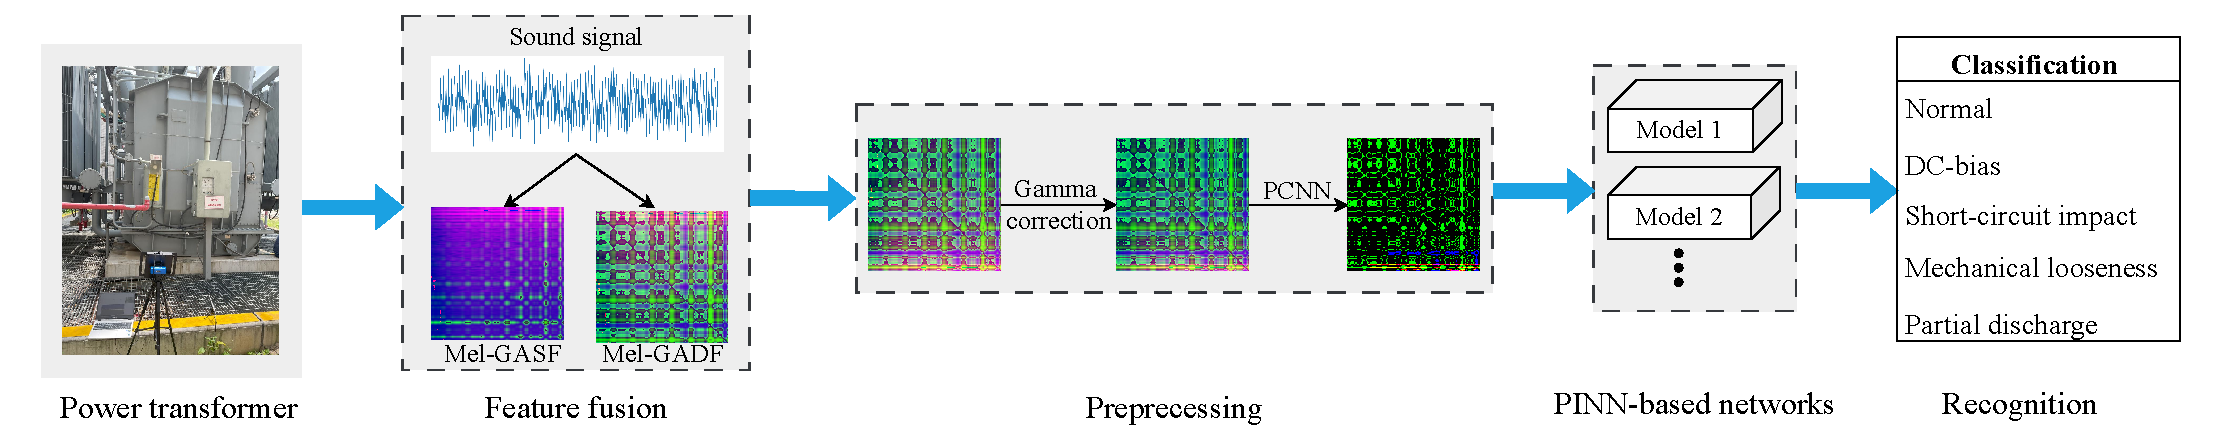
\includegraphics[width=1.0\linewidth]{drawing/pinn-alexnet/pinn-alexnet}
	\caption{Overall Framework of Transformer Faults Diagnosis.}
	\label{fig0}
\end{figure*}

\section{Time-Frequency Domain Representation}

\subsection{Mel Spectrogram}
\label{subsec1}
The Mel spectrogram effectively emulates the auditory characteristics of the human ear in speech recognition tasks \cite{WANG2026119319,10768989}. Since the human ear is more sensitive to low-frequency variations than to high-frequency changes, the Mel spectrogram transformers the original linear spectrogram into a logarithmic one \cite{SHAN2023112408,11097896}. The conversion formula is given by the following expression,
\begin{equation}
	f_{mel} = 2595 \lg\left(1 + \frac{f}{700}\right)
\end{equation}

\noindent where \( f \) represents the actual frequency, and \(f_{mel}\) is the corresponding frequency on the Mel scale. As the actual frequency increases, the converted frequency becomes progressively flatter, which aligns more closely with the auditory perception of the human ear. Therefore, this paper uses the Mel spectrogram as one of the two-dimensional feature maps for extraction. 

A 1-second transformer voiceprint signal was selected to generate a spectrogram, which was then processed using a Mel filter bank. The Mel filter bank consists of a set of triangular filters of equal height, with each filter's starting point positioned at the midpoint of the previous filter \cite{r1}. The corresponding frequencies on the Mel scale are linear. The Mel filter bank is defined as follows,
\begin{equation}
	H_m(k) = 
	\begin{cases} 
		0, & k < f(m-1) \\
		\frac{k - f(m-1)}{f(m) - f(m-1)}, & f(m-1) \leq k < f(m) \\
		1, & k = f(m) \\
		\frac{f(m+1) - k}{f(m+1) - f(m)}, & f(m) < k \leq f(m+1) \\
		0, & k > f(m+1)
	\end{cases}
\end{equation}

\noindent where \(H_m(k)\) represents the formula for the \(m\)-th filter, and \(f(m-1)\), \(f(m)\), and \(f(m+1)\) denote the starting point, midpoint, and ending point of the \(m\)-th filter, respectively. The Mel spectrogram obtained after filtering is shown in Fig.~\ref{fig1}.


\begin{figure}[htbp]
	\centering
	
	\begin{subfigure}[b]{0.45\textwidth}
		\centering
		\includegraphics[width=\textwidth]{Mel_Wave/Normal.png}
		\caption*{(a)} 
	\end{subfigure}
	\hfill
	
	\begin{subfigure}[b]{0.45\textwidth}
		\centering
		\includegraphics[width=\textwidth]{Mel_Wave/Mel_spectrogram.png}
		\caption*{(b)}
	\end{subfigure}
	
	\caption{Transformer in normal status. (a) Waveform of the voiceprint signal. (b) Corresponding Mel spectrogram.}
	\label{fig1}
\end{figure}

\subsection{Gramian Angular Field}
Gramian Angular Field (GAF) is a method that transforms and encodes time-series signals into images with rich feature information. Initially proposed for time-series classification using computer vision techniques \cite{10114345}. The method is described as follows \cite{10281942}.

\begin{enumerate}
	\item{for a time series}
	\begin{equation}
		X = \{x_1, x_2, \ldots, x_n\} \quad (n = 1, 2, 3\ldots)
	\end{equation}
	which is composed of the amplitudes at \(n\) moments.To facilitate the conversion between Cartesian and polar coordinates, the time series \(X\) is typically normalized using (4), ensuring that each value falls within the interval \([-1,1]\), resulting in the one-dimensional structured data \(\tilde{x}\) after normalization.
	
	\begin{equation}
		\tilde{x} = \frac{(x_i - \min X) + (x_i - \max X)}{\max X - \min X}
	\end{equation}
	\noindent The normalized \(X\) is denoted as \(\tilde {X}\).
	
	
	\item{Encode the value of \(\tilde{x}\) as a cosine angle, and represent it in polar coordinates as \(\phi_i\)} and \(r_i\), as shown in (5).
	
	\begin{equation}
		\begin{cases} 
			\phi_i = \arccos(\tilde{x}_i), & -1 \leq \tilde{x}_i \leq 1, \tilde{x}_i \in \tilde{X} \\
			r_i = \dfrac{i}{n}, & i = 1, \ldots, n 
		\end{cases}
	\end{equation}
	
	\noindent where \(\tilde{x}\) and \(r_i\) are the polar angle of point \(i\) and the polar radius of point \(i\).
	
	\item{Finally, the GAF can be calculated by using the sum (or difference) of the phase angles of the time series points after the polar coordinate transformation. Gramian angular fields are divided into two forms: the Gramian Angular Summation Field (GASF) \(\boldsymbol{G}_s\) and the Gramian Angular Difference Field (GADF) \(\boldsymbol{G}_d\). The specific calculations are shown in (6) and (7), respectively.

		\begin{equation}
			\resizebox{\linewidth}{!}{$
				\boldsymbol{G}_s = \begin{bmatrix}
					\cos(\phi_1 + \phi_1) & \cos(\phi_1 + \phi_2) & \cdots & \cos(\phi_1 + \phi_n) \\
					\cos(\phi_2 + \phi_1) & \cos(\phi_2 + \phi_2) & \cdots & \cos(\phi_2 + \phi_n) \\
					\vdots & \vdots & \ddots & \vdots \\
					\cos(\phi_n + \phi_1) & \cos(\phi_n + \phi_2) & \cdots & \cos(\phi_n + \phi_n)
				\end{bmatrix}
				$}
		\end{equation}
		
		\begin{equation}
			\resizebox{\linewidth}{!}{$
				\boldsymbol{G}_d = \begin{bmatrix}
					\sin(\phi_1 - \phi_1) & \sin(\phi_1 - \phi_2) & \cdots & \sin(\phi_1 - \phi_n) \\
					\sin(\phi_2 - \phi_1) & \sin(\phi_2 - \phi_2) & \cdots & \sin(\phi_2 - \phi_n) \\
					\vdots & \vdots & \ddots & \vdots \\
					\sin(\phi_n - \phi_1) & \sin(\phi_n - \phi_2) & \cdots & \sin(\phi_n - \phi_n)
				\end{bmatrix}
				$}
	\end{equation}}
	
\end{enumerate}

As illustrated in Fig.~\ref{fig2}, the signal collected from a transformer under normal conditions is transformed into GAF image \cite{8975572}, capturing the temporal dependencies and structural patterns of the signal over time.

\begin{figure}[!t]
	\centering
	\graphicspath{{GAF/}}
	\subfloat[]{\includegraphics[width=0.22\textwidth]{GASF}}\hfill
	\subfloat[]{\includegraphics[width=0.22\textwidth]{GADF}}
	\caption{Transformer vibration signals after GAF transformation: (a) GASF. (b) GADF.}
	\label{fig2}
\end{figure}

This paper selects five transformer conditions: normal, partial discharge, mechanical looseness, short-circuit impact and DC-bias and collects voiceprint signals for each condition. For each fault type, the voiceprint data for each 1-second interval is selected to generate a Mel spectrogram. Simultaneously, the data for this 1-second interval undergoes GAF transformation to obtain two types of time-frequency spectrograms: the GASF and GADF.


\section{Feature Extraction}
\subsection{Mel-GAF Feature Fusion}
The Mel spectrogram effectively represents the time-domain and frequency-domain relationship of the voiceprint signal. Meanwhile, applying the GAF transformation to the original data compensates for the low-frequency loss issue in the Mel spectrogram, resulting in a new two-dimensional time-frequency spectrogram. Feature fusion is a widely used technique in machine learning and deep learning, primarily aimed at combining feature information from different sources or levels to enhance the model's representational capacity and performance \cite{10902169,10856367}. 

In this study, feature fusion is applied prior to model input by concatenating features at the channel level to form a three-channel image. Specifically, Mel spectrogram features and GAF images are extracted and fused. Before fusion, all images are normalized and resized to a unified dimension. the GAF images are resized to \(224 \times 224\) pixels to match the dimensions of the Mel spectrogram. Additionally, the GAF images are converted to grayscale and normalized, allowing them to serve as an individual channel for fusion. This processing step ensures dimensional consistency and enables effective feature-level fusion during training.

\subsection{Image Preprocessing}
As shown in Fig.~\ref{fig3}(a), we observed that features of the Mel spectrogram became less prominent in the fused images. This is because, in the RGB fusion, the Mel spectrogram is assigned to the red (R) channel, which tends to lose visual saliency during RGB composition. To address this issue, we applied gamma correction to the fused images during preprocessing, enhancing its contrast and improving feature visibility \cite{11000314}. 

Gamma correction is a widely used nonlinear transformation technique in image processing, designed to adjust image contrast. It is especially effective for enhancing details in underexposed or overexposed regions. The transformation is typically defined as \cite{8362729}:
\begin{equation}
	I_{\text{out}} = c I_{\text{in}}^{\gamma}
\end{equation}
where \(\gamma\) is the gamma value, \(c\) is typically set to 1, and \(I_{\text{in}}\) and \(I_{\text{out}}\) represent the input and output pixel intensities, respectively, normalized to the range \([0,1]\). A gamma value less than 1 enhances darker regions, whereas a value greater than 1 emphasizes brighter areas. 

The transformer acoustic signals are primarily concentrated in the low-frequency range \cite{4712660}. Although the Mel spectrogram applies logarithmic compression, the dynamic range remains relatively large. When direct linear normalization is applied, low-frequency regions often appear dark and less distinguishable. To address this, gamma correction with \(\gamma=1.7\) is applied to enhance low-intensity regions while compressing high-intensity areas. This adjustment makes the low-energy frequency bands in the Mel spectrogram more visually prominent and textured, thereby improving the network's ability to learn subtle abnormal features in low-energy regions during training.

For each new pixel value in the target image, bicubic interpolation estimates the value based on 16 neighboring pixels from the source image using cubic polynomial interpolation \cite{9257189}. Compared to nearest-neighbor interpolation, which may cause the loss of structural lines, and bilinear interpolation, which often blurs texture boundaries, bicubic interpolation better preserves the fine textures and detailed structures present in images like Mel spectrogram and GAF representations. It is described as,
\begin{equation}
	P(x) = \sum_{i=-1}^{2} \sum_{j=-1}^{2} w(i,j) \cdot I(x+i, y+j)
\end{equation}

\noindent where the interpolation weight \(w(i,j)\), constructed via a cubic function, captures subtle pixel intensity variations and better preserves local structural trends.

Fig.~\ref{fig3} compares the fused images before and after gamma correction. In the original Mel-GADF image, the low-frequency regions appear relatively dark due to the wide dynamic range of amplitude, making it difficult to distinguish fine-grained fault-related features. After applying gamma correction with \(\gamma=1.7\), the contrast in low-energy regions is significantly enhanced, revealing more detailed textures and structural patters. This enhancement allows the model to better focus on subtle variations in the acoustic signals.


\begin{figure}[!t]
	\centering
	\graphicspath{{Mel-GAF-Noise/}}
	\subfloat[]{\includegraphics[width=0.22\textwidth]{1
	}}\hfill
	\subfloat[]{\includegraphics[width=0.22\textwidth]{2}}
	
	\caption{Comparison of Mel-GADF image before and after gamma correction. (a) Mel-GADF. (b) Gamma-corrected Mel-GADF with \(\gamma=1.7\)}
	\label{fig3}
\end{figure}


\subsection{Fused Images}

In the final RGB image, the R channel represents the Mel spectrogram energy, with intensity values scaled to the range of 0-255, while the green (G) channel contains the GAF-derived texture information. To incorporate complementary information, the differences between the Mel spectrogram and GAF features is computed and assigned to the red (B) channel. With this design, each RGB channel carries distinct and complementary information: the B channel reflects the differences between the two feature types. This channel-wise distinction facilitates the model's ability to learn synergistic and discriminative features more effectively. Moreover, it preserves the joint representation of both Mel and GAF time-frequency features during network training, aligning with the semantic objective of feature-level fusion. Overall, this design enhances the network's capacity to capture complementary patterns from both spectral energy and phase-based texture domains.

For RGB three-channel images, neural networks are capable of learning composite features across channels \cite{9673131}. In our fused images, the R, G, and B channels represent distinct types of features, with color encoding the underlying feature semantics. Therefore, we adopt a fixed fusion strategy as follows:

\begin{enumerate}
	\item{Unified Normalization and Channel Assignment: Both the Mel spectrogram and GAF images are independently normalized to the range [0,1] to insure consistent input scaling. The R channel encodes the Mel spectrogram energy, the G channel represents the GAF-derived texture features, and the B channel capture the pixel-wise difference between the Mel and GAF image. highlighting complementary information between the two modalities.}
	\item{Consistent Gamma Correction: Gamma correction is uniformly applied across all image samples to enhance feature contrast and improve the perceptibility of details, particularly in low-intensity or dark regions. This preprocessing step contributes to better feature discrimination during model training.}
\end{enumerate}

Fig.~\ref{fig4} shows the transformer under five different conditions: normal, DC-bias, short-circuit impact, mechanical looseness and partial discharge. The corresponding feature representations are Mel-GASF, Mel-GADF, and Mel spectrogram. the Integrating the Mel spectrogram with the GAF image enables the deep learning model to extract a more comprehensive representation of the transformer signal. This fusion effectively captures both local frequency variation patterns and the global temporal structure of the underlying time series.

\begin{figure*}[htbp]
	\centering
	\graphicspath{{MEL-GASF/}{MEL-GADF/}{MEL/}}
	
	\begin{tabular}{c@{\hspace{0.3cm}}ccccc}
		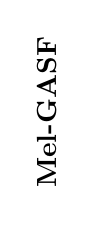
\begin{tikzpicture}
			\node[align=right] {\rotatebox{90}{\textbf{Mel-GASF}}};
		\end{tikzpicture}
		
		\includegraphics[width=0.15\textwidth]{Normal_part0} &
		\includegraphics[width=0.15\textwidth]{G4_10pSeventhHarmonic_1} &
		\includegraphics[width=0.15\textwidth]{DCBias2_1} &
		\includegraphics[width=0.15\textwidth]{Loosen1_1} &
		\includegraphics[width=0.15\textwidth]{PartialDischarge1_1} \\
	\end{tabular}
	
	\vspace{0.15cm}
	\begin{tikzpicture}
		\draw[dash pattern=on 8pt off 2pt, line width=0.6pt,blue] (0,0) -- (\textwidth,0);
		
	\end{tikzpicture}
	\vspace{0.15cm}
	
	
	\begin{tabular}{c@{\hspace{0.3cm}}ccccc}
		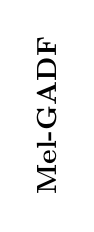
\begin{tikzpicture}
			\node[align=right] {\rotatebox{90}{\textbf{Mel-GADF}}}; 
		\end{tikzpicture}
		\includegraphics[width=0.15\textwidth]{Normal_part0_1} &
		\includegraphics[width=0.15\textwidth]{G4_10pSeventhHarmonic_1_1} &
		\includegraphics[width=0.15\textwidth]{DCBias2_1_1} &
		\includegraphics[width=0.15\textwidth]{Loosen1_1_1} &
		\includegraphics[width=0.15\textwidth]{PartialDischarge1_1_1} \\
	\end{tabular}
	
	
	\vspace{0.15cm}
	\begin{tikzpicture}
		
		\draw[dash pattern=on 8pt off 2pt, line width=0.6pt,blue] (0,0) -- (\textwidth,0);
	\end{tikzpicture}
	\vspace{0.15cm}
	
	
	\begin{tabular}{c@{\hspace{0.3cm}}ccccc}
		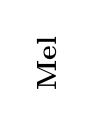
\begin{tikzpicture}
			\node[align=right] {\rotatebox{90}{\textbf{Mel}}};
		\end{tikzpicture}
		\subfloat[]{\includegraphics[width=0.15\textwidth]{Normal_Mel.png}} &
		\subfloat[]{\includegraphics[width=0.15\textwidth]{Harmonic_Mel.png}} &
		\subfloat[]{\includegraphics[width=0.15\textwidth]{DCBias_Mel.png}} &
		\subfloat[]{\includegraphics[width=0.15\textwidth]{Loosen_Mel.png}} &
		\subfloat[]{\includegraphics[width=0.15\textwidth]{PartialDischarge_Mel.png}} \\
	\end{tabular}
	
	\caption{Mel, Mel-GASF, and Mel-GADF spectrum between the real and fault acoustic signals for different operational statuses. (a) Normal, (b) DC-bias, (c)Short-circuit impact, (d) Mechanical looseness, and (e) Partial discharge.}
	\label{fig4}
\end{figure*}

\subsection{PCNNs-Based Processing}
Pulse-Coupled Neural Networks (PCNNs) are a type of neutral network model inspired by the biological visual system \cite{4305279,6338347}. Unlike conventional convolutional neural networks (CNNs), PCNNs emulate the spike firing mechanism of biological neurons \cite{10341267}. Neurons in PCNNs are interconnected through local receptive fields, exhibiting both self-excitation and lateral coupling characteristics. Due to these biologically inspired dynamics, PCNNs have been widely applied in image processing tasks such as image segmentation, edge detection, and feature extraction \cite{10848019}.
\noindent For each pixel location \((i, j)\), a PCNN typically comprises the following three core components:

\begin{enumerate}
	\item{Input Module} 
	\begin{equation}
		F_{i,j}[n] = e^{-\alpha_{F}} F_{i,j}[n - 1] + V_{F} S_{i,j}
	\end{equation}
	where \(S_{i,j}\) denotes the grayscale value of the pixel at location \((i, j)\) in the input image, \(\alpha_{F}\) is the decay constant, \(V_{F}\) represent the input gain coefficient, and \(F_{i,j}[n]\)  denotes the input stimulus at the \(n\)-th iteration.
	
	\item{Linking Module}
	\begin{equation}
		L_{i,j}[n] = e^{-\alpha_L} L_{i,j}[n-1] + V_L \sum_{k,l} W_{i,j;k,l} Y_{k,l}[n-1]
	\end{equation}
	
	where \(L_{i,j}\) denotes the coupling input at pixel \((i, j)\) at iteration \(n\), which aggregates the pulsed outputs (0 or 1) from neighboring neurons in the previous step. \(W_{i,j;k,l}\) represents the coupling weight between pixel \((i, j)\) and its neighboring pixel \((k, l)\), typically defined by a local Gaussian kernel.
	
	\item{Internal Activity and Dynamic Threshold Modules}
	
	\begin{equation}
		U_{i,j}[n] = F_{i,j}[n] (1 + \beta L_{i,j}[n])
	\end{equation}
	
	\begin{equation}
		Y_{i,j}[n] = 
		\begin{cases} 
			1, & \text{if } U_{i,j}[n] > T_{i,j}[n] \\
			0, & \text{otherwise}
		\end{cases}
	\end{equation}
	
	\begin{equation}
		T_{i,j}[n] = e^{-\alpha_T} T_{i,j}[n-1] + V_T Y_{i,j}[n]
	\end{equation}
	
	where \(Y_{i,j}\) denotes the output pulse of neural at pixel \((i, j)\) at iteration \(n\), \(T_{i,j}[n]\) is the corresponding dynamic threshold, and \(U_{i,j}[n]\) represents the total internal excitation.
\end{enumerate}

Fig.~\ref{fig5} illustrates the enhanced feature maps obtained by applying PCNNs to each RGB channel of the Mel-GADF images under normal operation conditions, followed by normalization. As shown in the figure, with a fixed number of pulse iterations, increasing the initial threshold results in stronger suppression of background noise. Notably, when the threshold is set to 1.0, the output image becomes entirely black due to complete inhibition of neuronal firing. To achieve a balance between preserving fine details and suppressing background noise, a threshold value of 0.8 is selected in this study. The application of PCNNs significantly enhances feature quality by effectively reducing noise in the input representations.

\begin{figure}[!t]
	\centering
	\graphicspath{{VT/}}
	\subfloat[]{\includegraphics[width=0.22\textwidth]{Normal_part0}}\hfill
	\subfloat[]{\includegraphics[width=0.22\textwidth]{Normal_part04}}\hfill
	\subfloat[]{\includegraphics[width=0.22\textwidth]{Normal_part06}}\hfill
	\subfloat[]{\includegraphics[width=0.22\textwidth]{Normal_part08}}
	
	\caption{Mel-GADF image after PCNNs processing with different initial thresholds. (a) Original image without processing; (b-d) Results with thresholds set to 0.4, 0.6, and 0.8, respectively.}
	\label{fig5}
\end{figure}


\section{Improved PINNs for Fault Diagnosis}
\subsection{PINN-Based Neutral Networks}
Physics-Informed Neural Networks (PINNs) integrate physical laws into neural network architectures, enabling collaborative modeling of both data-driven patterns and underlying physical mechanisms \cite{9903391,r4}. By incorporating domain-specific constraints, such as partial differential equations (PDEs) or boundary conditions, PINNs can make accurate predictions even when data is sparse or incomplete \cite{11047028,10337737}. Due to their strong generalization ability under physical priors, PINNs have found widespread applications in scientific computing, engineering analysis, climate modeling, and biomechanics \cite{10729277}. 

The core principle of PINNs lies in the integration of physics-based constraints directly into the training process. Unlike traditional neural networks that rely solely on data-driven supervision through labeled samples, PINNs are additionally guided by the governing physical laws---such as partial differential equations (PDEs)---thereby improving model generalization, stability, and interpretability \cite{s1}.

While conventional neural networks approximate target functions by minimizing empirical loss, PINNs incorporate physical models as additional soft constraints into the loss function. A general form of the governing PDE in the context of PINNs can be written as: 
\begin{equation}
	\label{eq1}
	\mathcal{D}[u(\mathbf{x}, t)] = s(\mathbf{x}, t)
\end{equation}

\noindent where \(\mathbf{x} \in \mathbb{R}^d\) represents spatial coordinates, \(t \in \mathbb{R}\) denotes time, \(u(\mathbf{x}, t)\) is the unknown solution to be approximated, \(\mathcal{D}[\cdot]\) is a differential operator representing the physical law, and \(s(\mathbf{x}, t)\) is a known source or forcing function.

The PINNs framework comprises a neural network that takes space-time coordinates \((\mathbf{x}, t)\) as input, corresponding to the initial conditions (ICs) and boundary conditions (BCs). The network output \(\hat{u}(\mathbf{x}, t)\) serves as an approximation of the true solution \({u}(\mathbf{x}, t)\), and is obtained by sequential application of learnable weights $\boldsymbol{W}$, bias $\boldsymbol{b}$, and nonlinear activation function \(\sigma(\cdot)\). Specifically, each neuron computes a weighted sum of its inputs plus a bias, followed by an activation operation. To evaluate the PDE constraints, automatic differentiation (AD) is employed to compute space-time derivatives of \(\hat{u}(\mathbf{x}, t)\) at randomly sampled collocation points (CPs) within the domain. These CPs are used to calculate the residual of the PDE, which becomes part of the loss function minimized during training. Fig.~\ref{fig6} illustrates the overall PINNs architecture. The total loss function consists of three components: the loss over initial conditions \(\mathcal{L}_{\mathrm{IC}}\), boundary conditions \(\mathcal{L}_{\mathrm{BC}}\), and the PDE residual \(\mathcal{L}_{\mathrm{R}}\), expressed as:

\begin{equation}
	\mathcal{L}(\boldsymbol{\theta}) = \mathcal{L}_{\mathrm{IC}}(\boldsymbol{\theta}) + \mathcal{L}_{\mathrm{BC}}(\boldsymbol{\theta}) + \mathcal{L}_{\mathrm{R}}(\boldsymbol{\theta})
\end{equation}

\noindent where \(\boldsymbol{\theta} = \{\boldsymbol{W}, \boldsymbol{b}\}\) denotes the trainable parameters of the network. The individual loss components are defined as follows:
\begin{equation}
	\mathcal{L}_{\mathrm{IC}}(\boldsymbol{\theta}) = \frac{1}{N_\mathrm{IC}} \sum_{i=1}^{N_\mathrm{IC}} \left| \hat{u}(\mathbf{x}_i, 0) - u(\mathbf{x}_i, 0) \right|^2 \
\end{equation}

\begin{equation}
	\mathcal{L}_{\mathrm{BC}}(\boldsymbol{\theta}) = \frac{1}{N_{\mathrm{BC}}} \sum_{i=1}^{N_{\mathrm{BC}}} \left| \hat{u}(\mathbf{x}_i, t_i) - u(\mathbf{x}_i, t_i) \right|^2 \
\end{equation}

\begin{equation}
	\mathcal{L}_{\mathrm{R}}(\boldsymbol{\theta}) = \frac{1}{N_{\mathrm{R}}} \sum_{i=1}^{N_{\mathrm{R}}} \left| r(\mathbf{x}_i, t_i) \right|^2
\end{equation}

Here, \(N_\mathrm{IC}\), \(N_\mathrm{BC}\), and \(N_\mathrm{R}\) are the number of sample points used for initial condition, boundary condition, and residual loss, respectively. The residual \(r(\mathbf{x}, t)\) is derived from the PDE definition in (\ref{eq1}), and is expressed as:

\begin{equation}
	r(\mathbf{x}, t) = \mathcal{D}[\hat{u}(\mathbf{x}, t)] - s(\mathbf{x}, t)
\end{equation}

This residual quantifies the deviation of the network output from satisfying the governing physical law at each collocation point and is minimized to embed physical fidelity into the learned solution.

\begin{figure}
	\centering
	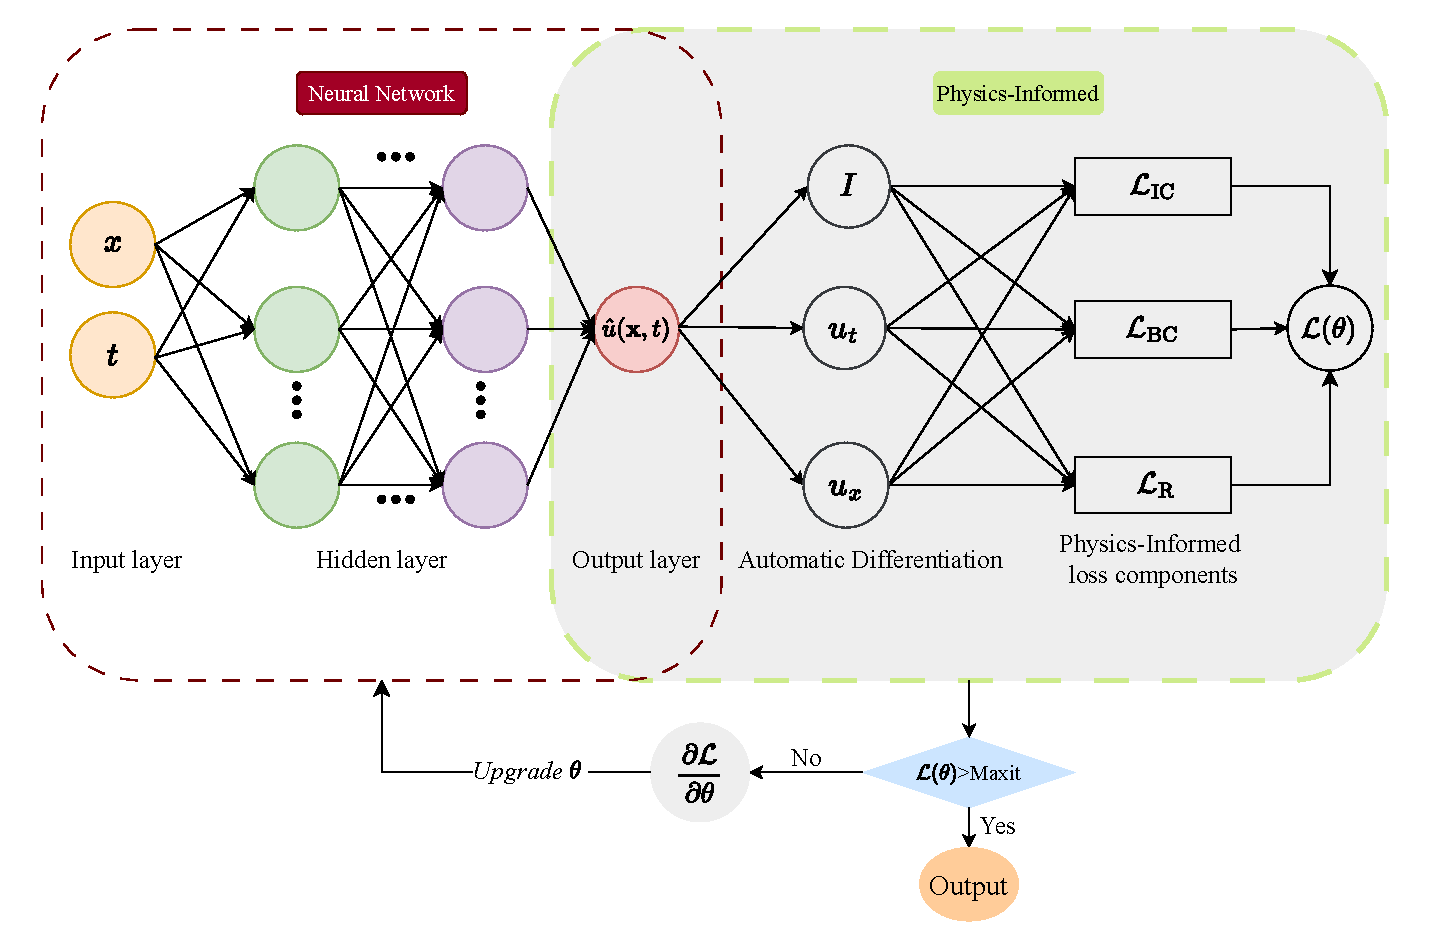
\includegraphics[width=1.0\linewidth]{drawing/PINN/pinn1}
	\caption{Flowchart of the physics-informed neural networks (PINNs).}
	\label{fig6}
\end{figure}


To enhance the model's awareness of physical pattern, an improved PINNs framework is proposed, where physical consistency is introduced as  a regularization constraint. On the Mel spectrogram, a heat diffusion-inspired prior is enforced by assuming the Laplace equation holds approximately:
\begin{equation}
	\Delta u(x, y) \approx 0
\end{equation}

This physical prior leads to the formulation of a Laplacian regularization loss, which encourage local smoothness in the predicted feature maps \cite{10908022}. The incorporation of this loss significantly improves the model's generalization capability and physical plausibility. In scenarios with limited or noisy data, the use of physics-based regularization also mitigates overfitting. Specifically, Laplacian smoothness is applied in the image space, where the underlying physical intuition is that fault-induced patterns are expected to exhibit localized irregularities or "disturbances" along the frequency and time dimensions, while non-fault patterns should remain relatively smooth \cite{7010929}. Within this framework, the PINNs model acts as a saliency extractor, highlighting spatial regions associated with physically meaningful anomalies. These salient regions may correspond to time segments that reflect abnormal behaviors in the acoustic signal. To further enhance interpretability and physical reliability, the extracted physical field is fed back into the final classification layer, enabling the model to incorporate physical awareness directly into the decision-making process. This feedback mechanism encourages the network to focus on regions that satisfy physical consistency, thereby improving its ability to detect fault-related anomalies in a more robust and physically interpretable manner.

\subsection{Fault Classification and Diagnosis Module}
To evaluate the applicability and effectiveness of the extracted features from acoustic signal samples, a fault diagnosis module is integrated into the proposed framework. In this study, four widely adopted CNN architectures are selected as backbone classifiers within the PINN framework: LeNet, ResNet, ConvNeXt, and AlexNet. The rationale for employing multiple classification backbones is to comprehensively assess the performance and generalizability of the feature extraction strategy under varying model complexities and architectural designs. This approach ensures a more robust and fair evaluation across different types of deep learning classifiers. The details of each classifier are summarized as follows:
\begin{enumerate}
	\item{The original LeNet is adapted to process \({224\times224}\) grayscale acoustic spectrograms by expanding the input size from \({32\times32}\) and replacing the original tanh activation with ReLU for better convergence. A \(1\times 1\) convolutional layer is appended to generate physical-domain feedback, followed by a fully connected structure redesigned with a 64-unit bottleneck before the final classification output.}
	
	\item{To accommodate single-channel inputs, the standard ResNet-18 is modified by adjusting the first convolutional layer to accept 1-channel data and reducing the number of filters across the network. The residual block structure is preserved, but the channel sizes are scaled down to reduce model complexity. A \(1\times 1\) convolutional physics output layer is added to extract physical constraints from the feature maps, followed by an adaptive average pooling and a fully connected classifier suited for five-class classification.}
	
	\item{A lightweight version of ConvNeXt is implemented to balance performance and efficiency for fault diagnosis. The model uses a reduced number of blocks per stage and a simplified channel progression. All convolutions are adapted for 1-channel input, and only one block is retained in each stage. A physics output layer is inserted before the classifier to preserve physical interpretability, and an adaptive pooling layer is used to normalize spatial dimensions before the final fully connected layer.}
	
	\item{The classic AlexNet is redesigned with smaller convolutional kernels, batch normalization, and squeeze-and-excitation (SE) attention modules following each convolution to recalibrate channel-wise feature responses. The input channel is adjusted for grayscale spectrograms, and the feature maps are downsampled using max-pooling layers. After convolutional stages, an adaptive average pooling layer ensures fixed-size output, followed by a physics output layer for physical feedback, and a two-layer fully connected classifier tailored for multi-class fault classification.}
\end{enumerate}

Details of the modified network configurations are listed in Table~\ref{tab1}, highlighting the structural adjustments made in this study.

\begin{table*}[htbp]
	\centering
	\caption{Network Architecture of Modules (Enhanced for PINNs)}
	\label{tab1}
	\begin{tabular}{@{}llccccc@{}}
		\toprule
		
		\textbf{Module} & \textbf{Layer} & \textbf{Input size (C$\times$H$\times$W)} & \textbf{Kernel size} &  \textbf{Stride} & \textbf{Channels} & \textbf{Output size (C$\times$H$\times$W)} \\
		\midrule
		
		\multirow{7}{*}{\textbf{LeNet}} 
		&Conv1        & 1$\times$224$\times$224 & 5$\times$5 & 1  & 6   & 6$\times$224$\times$224 \\
		&ReLU1         & 6$\times$224$\times$224  & --          & --     & 6        & 6$\times$224$\times$224 \\
		&AvgPool1      & 6$\times$224$\times$224  & 2$\times$2  & 2      & 6        & 6$\times$112$\times$112 \\
		&Conv2         & 6$\times$112$\times$112  & 5$\times$5  & 1      & 16       & 16$\times$108$\times$108 \\
		&ReLU2         & 16$\times$108$\times$108 & --          & --     & 16       & 16$\times$108$\times$108 \\
		&AvgPool2      & 16$\times$108$\times$108 & 2$\times$2  & 2      & 16       & 16$\times$54$\times$54 \\
		&Phys\_Out     & 16$\times$54$\times$54   & 1$\times$1  & 1      & 1        & 1$\times$54$\times$54 \\
		\midrule
		
		\multirow{9}{*}{\textbf{ResNet}} 
		&Conv1         & 1$\times$224$\times$224  & 7$\times$7  & 2      & 32            & 32$\times$112$\times$112 \\
		&BN + ReLU     & 32$\times$112$\times$112 & --          & --     & 32            & 32$\times$112$\times$112 \\
		&MaxPool       & 32$\times$112$\times$112 & 3$\times$3  & 2      & 32            & 32$\times$56$\times$56 \\
		&BasicBlock1   & 32$\times$56$\times$56   & 3$\times$3  & 1      & 64 & 64$\times$56$\times$56 \\
		&BasicBlock2   & 64$\times$56$\times$56   & 3$\times$3  & 2      & 128 & 128$\times$28$\times$28 \\
		&BasicBlock3   & 128$\times$28$\times$28  & 3$\times$3  & 2      & 256 & 256$\times$14$\times$14 \\
		&BasicBlock4   & 256$\times$14$\times$14  & 3$\times$3  & 2      & 256            & 256$\times$7$\times$7 \\
		&Phys\_Out     & 256$\times$7$\times$7    & 1$\times$1  & 1      & 1              & 1$\times$7$\times$7 \\
		&AvgPool       & 256$\times$7$\times$7    & Adaptive    & --     & 256            & 256$\times$1$\times$1 \\
		\midrule
		
		\multirow{10}{*}{\textbf{ConvNeXt}} 
		&Stem Conv     & 1$\times$224$\times$224 & 4$\times$4  & 4      & 96              & 96$\times$56$\times$56 \\
		&Stage 1       & 96$\times$56$\times$56  & 3$\times$3  & 1      & 96              & 96$\times$56$\times$56 \\
		&Downsample1   & 96$\times$56$\times$56  & 2$\times$2  & 2      & 192             & 192$\times$28$\times$28 \\
		&Stage 2       & 192$\times$28$\times$28 & 3$\times$3  & 1      & 192             & 192$\times$28$\times$28 \\
		&Downsample2   & 192$\times$28$\times$28 & 2$\times$2  & 2      & 384             & 384$\times$14$\times$14 \\
		&Stage 3       & 384$\times$14$\times$14 & 3$\times$3  & 1      & 384             & 384$\times$14$\times$14 \\
		&Downsample3   & 384$\times$14$\times$14 & 2$\times$2  & 2      & 768             & 768$\times$7$\times$7 \\
		&Stage 4       & 768$\times$7$\times$7   & 3$\times$3  & 1      & 768             & 768$\times$7$\times$7 \\
		&Phys\_Out     & 768$\times$7$\times$7   & 1$\times$1  & 1      & 1               & 1$\times$7$\times$7 \\
		&AvgPool       & 768$\times$7$\times$7   & Adaptive    & --     & 768             & 768$\times$1$\times$1 \\
		\midrule
		
		\multirow{10}{*}{\textbf{AlexNet-SE}} 
		&Conv1        & 1$\times$224$\times$224 & 5$\times$5  & 2      & 16               & 16$\times$112$\times$112 \\
		&BN + ReLU + SE & 16$\times$112$\times$112 & --       & --     & 16               & 16$\times$112$\times$112 \\
		&MaxPool1     & 16$\times$112$\times$112 & 2$\times$2 & 2      & 16               & 16$\times$56$\times$56 \\
		&Conv2        & 16$\times$56$\times$56  & 3$\times$3  & 1      & 32               & 32$\times$56$\times$56 \\
		&BN + ReLU + SE & 32$\times$56$\times$56 & --       & --     & 32               & 32$\times$56$\times$56 \\
		&MaxPool2     & 32$\times$56$\times$56  & 2$\times$2 & 2      & 32               & 32$\times$28$\times$28 \\
		&Conv3        & 32$\times$28$\times$28  & 3$\times$3  & 1      & 48               & 48$\times$28$\times$28 \\
		&BN + ReLU + SE & 48$\times$28$\times$28 & --       & --     & 48               & 48$\times$28$\times$28 \\
		&AdaptiveAvgPool & 48$\times$28$\times$28 & --       & --     & 48               & 48$\times$4$\times$4 \\
		&Phys\_Out    & 48$\times$4$\times$4     & 1$\times$1  & 1      & 1                & 1$\times$4$\times$4 \\
		\bottomrule
	\end{tabular}
\end{table*}


\section{Experimental Setup and Result}
\subsection{Data Collection and Description}
In this study, an experimental platform was established to capture raw acoustic signals emitted by power transformers at an operational substation, which includes multiple transformers distributed across different locations. At the vicinity of a 220 kV transformer---where vibration-induced acoustic emissions are relatively prominent---data acquisition equipment was deployed approximately 1.2 meters in front of the transformer. As illustrated in Fig.~\ref{fig7}, the acquisition setup comprises an omnidirectional microphone, a tripod, and a USB cable for both signal transmission and power supply. The collected acoustic signals were categorized into five distinct classes, corresponding to different transformer operating conditions:
\begin{itemize}
	\item{Normal (N0),}
	\item{Short-circuit impact (N1),}
	\item{DC-bias (N2),}
	\item{Mechanical looseness (N3), and}
	\item{Partial Discharge (N4),}
\end{itemize}
as summarized in Table~\ref{tab2}.

\begin{table}[]
	\centering
	\caption{Samples of Transformer Operating Conditions}
	\label{tab2}
	\begin{tabular}{{p{1.2cm}p{3.2cm}c}}
		\toprule
		Class label & Description of different \newline
		operational statuses & Sample number \\
		\midrule
		N0 & Normal          & 185 \\
		N1 & Short-circuit impact           & 119 \\
		N2 & DC-bias           & 119 \\
		N3 & Mechanical looseness   & 119 \\
		N4 & Partial discharge   & 119 \\
		\bottomrule
	\end{tabular}
\end{table}




For model training and evaluation, all audio recordings were resampled to a uniform sampling rate of 44.1kHz, segmented into 1-second clips, and saved in .WAV format. The resulting dataset was randomly split into training (80\%), validation (10\%), and test (10\%) sets as shown in Table~\ref{tab3}, to ensure a balanced and robust experimental setup.


\begin{table}[htbp]
	\centering
	\caption{Composition of The Experimental Dataset}
	\label{tab3}
	\begin{tabular}{l c c c c c c }
		\toprule
		\multirow{2}{*}{Datasets} & 
		\multirow{2}{*}{Total} & 
		\multicolumn{5}{c}{Sample number of different classes} \\
		\cmidrule(lr){3-7}
		&  & N0 & N1 & N2 & N3 & N4  \\
		\midrule
		Traning set & 520 & 148 & 83 & 98 & 92 & 99 \\
		Validating set & 65 & 13 & 17 & 10 & 13 & 12 \\
		Testing set &  66& 24 & 9 & 11 & 14 & 8 \\
		\bottomrule
	\end{tabular}
\end{table}


\begin{figure}[!t]
	\centering
	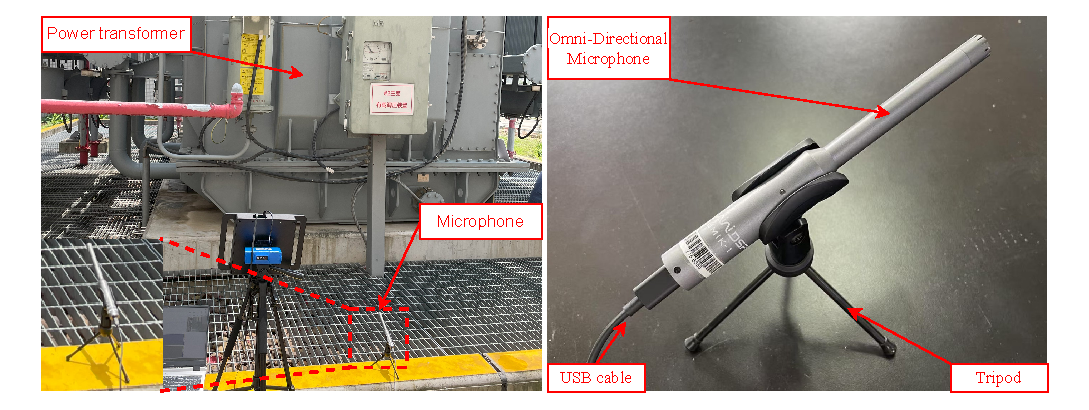
\includegraphics[width=1.0\linewidth]{equipment/采集设备}
	\caption{Experimental platform of acoustic signal acquisition.}
	\label{fig7}
\end{figure}

The overall feature extraction processing is shown in Fig.~\ref{fig8}.
\begin{figure*}
	\centering
	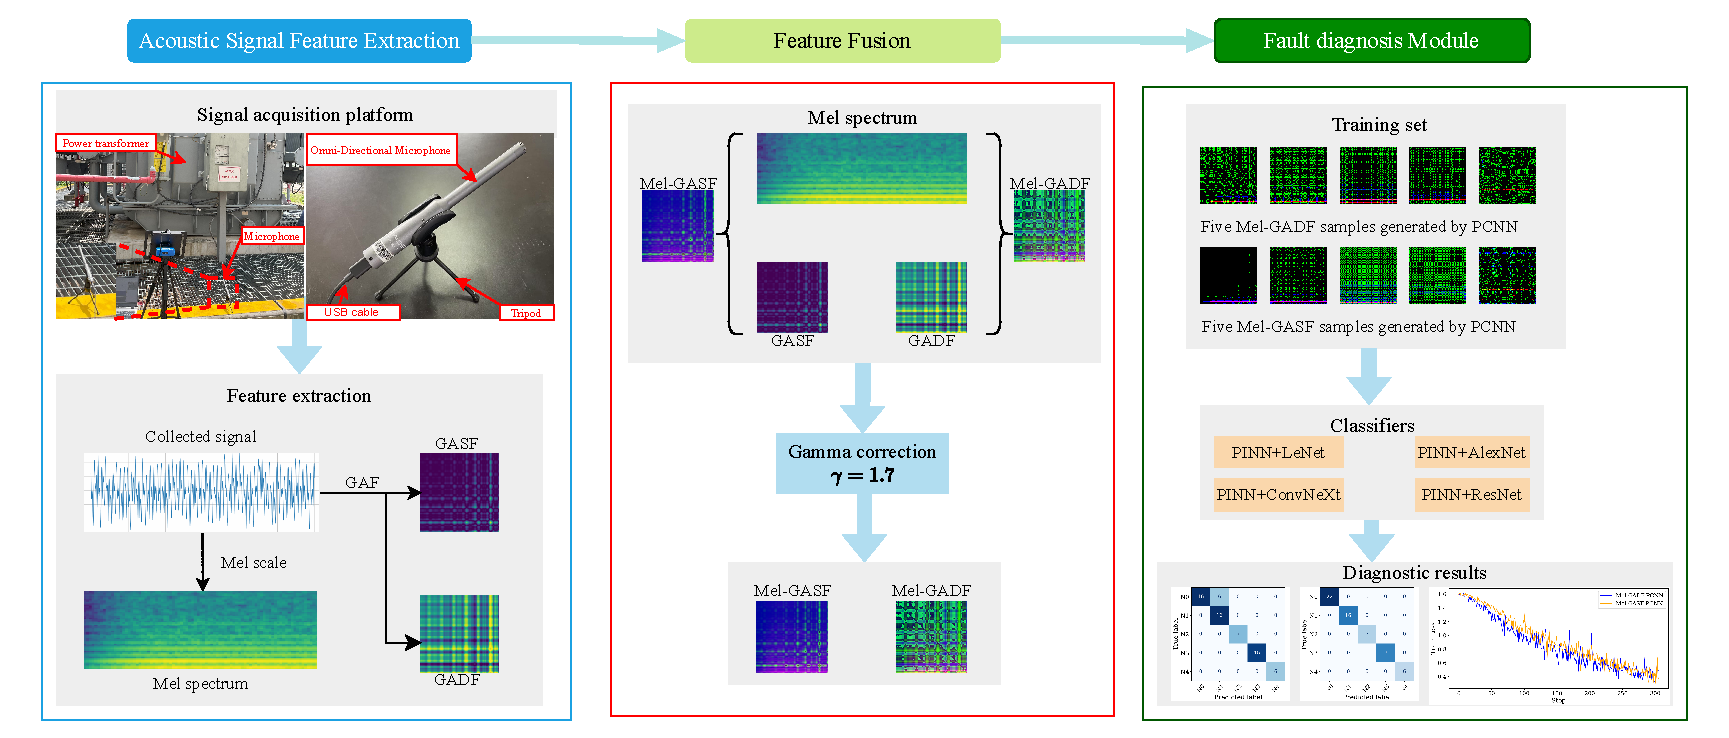
\includegraphics[width=1.0\linewidth]{drawing/overall/overall}
	\caption{Overall Framework of Transformer Faults Diagnosis Based on Improved PINNs.}
	\label{fig8}
\end{figure*}

The experiments in this study were conducted on a system equipped with an Intel i9-14900K CPU and an NVIDIA RTX 5090 GPU. The software environment was based on PyTorch 2.7 and CUDA 12.8.


\subsection{Evaluation Metrics}
To comprehensively evaluate the performance of the different models, multiple metrics were employed. In addition to accuracy and geometric mean, we also computed the precision and \(F_1\) score for each class. Furthermore, the standard deviation of these metrics across different classes was calculated to assess the consistency of the model's performance, denoted as \(\sigma_{\text{Precision}}\), \(\sigma_{\text{Recall}}\), and \(\sigma_{F_1}\), respectively. These standard deviation metrics provide insights into the stability and robustness of the model across different fault categories, where lower values indicate more uniform classification performance.

\begin{equation}
	\text{Accuracy} = \frac{\sum_{i=1}^{K} TP_i}{\sum_{i=1}^{K} (TP_i + FP_i + FN_i)}
\end{equation}

where \(TP_i\), \(FP_i\), and \(FN_i\) represent the number of true positive, true negative, false positive, and false negative samples, respectively. The accuracy measures the overall proportion of correctly classified samples.

\begin{equation}
	\text{Precision} = \sum_{i=1}^{K} w_i \cdot \frac{TP_i}{TP_i + FP_i}
\end{equation}

\begin{equation}
	\text{Recall} = \sum_{i=1}^{K} w_i \cdot \frac{TP_i}{TP_i + FN_i}
\end{equation}

\begin{equation}
	F_1 = \sum_{i=1}^{K} w_i \cdot \frac{2 \cdot \text{Precision}_i \cdot \text{Recall}_i}{\text{Precision}_i + \text{Recall}_i}
\end{equation}

where \( w_i = \frac{n_i}{\sum_{j=1}^{K} n_j} \) denotes the proportion of samples in class \( i \), and \(n_i\) is the number of samples in class \(i\).

\begin{equation}
	G_{\text{mean}} = \left( \prod_{i=1}^{K} \frac{TP_i}{TP_i + FN_i} \right)^{\frac{1}{K}}
\end{equation}

G-Mean reflects the balance of classification performance across all classes.

\begin{align}
	\sigma_{\text{Precision}} &= \sqrt{ \frac{1}{K} \sum_{i=1}^{K} \left( \text{Precision}_i - \bar{\text{Precision}} \right)^2 } \\
	\sigma_{\text{Recall}} &= \sqrt{ \frac{1}{K} \sum_{i=1}^{K} \left( \text{Recall}_i - \bar{\text{Recall}} \right)^2 } \\
	\sigma_{F_1} &= \sqrt{ \frac{1}{K} \sum_{i=1}^{K} \left( F_{1,i} - \bar{F_1} \right)^2 }
\end{align}

where the values of \(F_1\) score and \(G_{\text{mean}}\) ranges from 0 to 1. 


Fig.~\ref{fig9} illustrates the training loss trends of the Mel-GASF-PCNN and Mel-GADF-PCNN features under the AlexNet-SE network. Overall, both feature types exhibit a clear downward trend, indicating successful model training. 

\begin{figure}
	\centering
	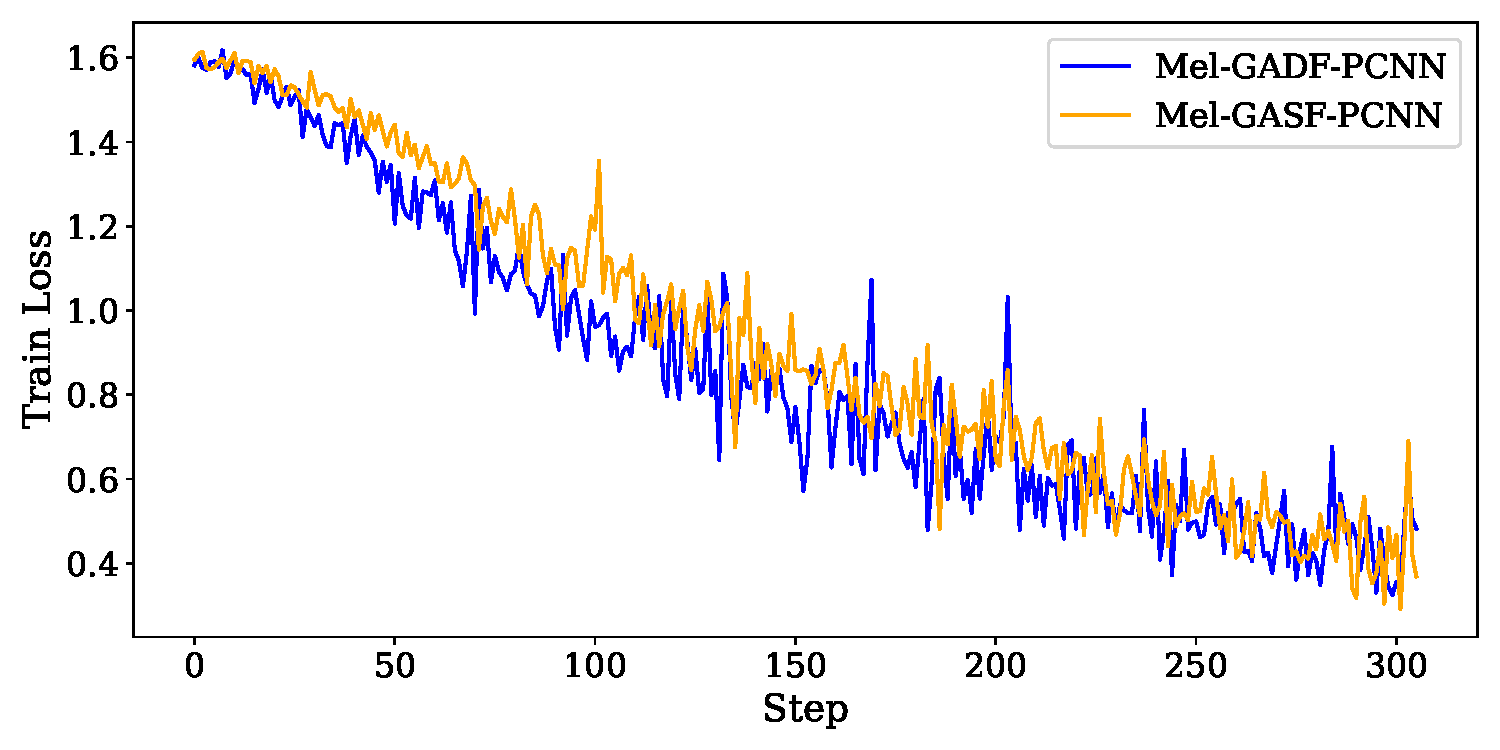
\includegraphics[width=1.0\linewidth]{curve/compare_loss_curve2}
	\caption{Comparison of training loss curve for Mel-GADF-PCNN and Mel-GASF-PCNN features using the AlexNet-SE network.}
	\label{fig9}
\end{figure}

According to the evaluation results on the test set, the Mel-GADF features outperform Mel-GASF across multiple classification performance metrics. Specifically, Mel-GADF achieved slightly higher values in accuracy ($93.94\%$), weighted recall ($93.94\%$), $F_1$ (0.9392), and \(G_{mean}\) (0.9587). The improvement in \(G_{mean}\) is particularly notable, indicating that Mel-GADF yields a more balanced classification performance across all categories.

In addition, the standard deviation metrics further reveal the classification stability of each feature type. Mel-GADF shows significantly lower standard deviations compared to Mel-GASF, especially in \(\sigma_{F_1}\), which is only 0.0434 (versus 0.1490 for Mel-GASF). This suggest that Mel-GADF provides more consistent and stable classification results, demonstrating better generalization capability.

In summary, although Mel-GASF features exhibit better convergence behavior during training, Mel-GADF features show stronger generalization and more stable multi-class fault recognition performance during testing. Therefore, within the proposed model framework, Mel-GADF is more suitable as the input feature for transformer acoustic image classification. Fig.~\ref{fig10} presents the overall workflow of the proposed transformer faults diagnosis method.

\begin{figure}
	\centering
	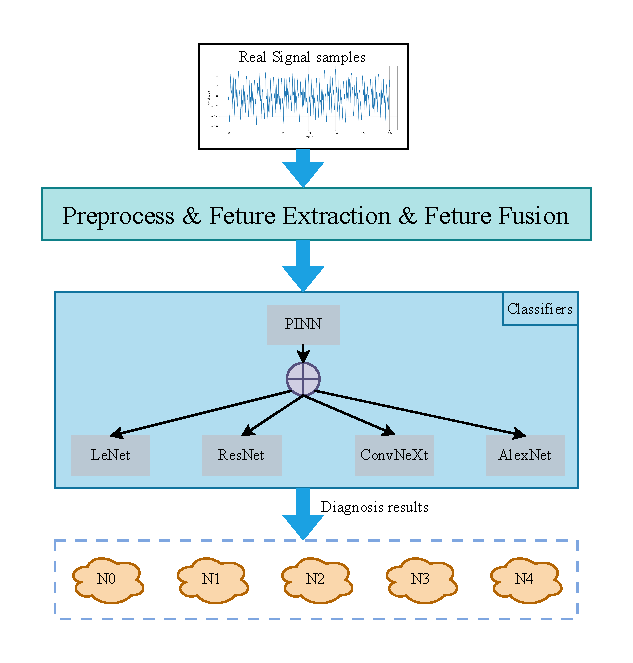
\includegraphics[width=1.0\linewidth]{drawing/fault-diagnosis/structure}
	\caption{Structure of fault diagnosis module.}
	\label{fig10}
\end{figure}

As shown in Table IV, the use of the PCNN network for further feature extraction has significantly improved the model's performance, particularly in key metrics such as accuracy and precision. Additionally, the model's stability has been enhanced, as indicated by the reduction in standard deviation. This suggests that PCNN is an effective approach for improving feature extraction.

\begin{table*}[]
	\centering
	\label{tab4}
	\caption{Fault classification results for four features using different models.}
	\begin{tabular}{l l c c c c c c c c c}
		\toprule
		\multirow{2}{*}{Feature} & \multirow{2}{*}{Model} & \multicolumn{6}{c}{Fault multi-classification evaluation index}\\
		\cmidrule(lr){3-9}	
		&  & Accuracy(\%) & Precision(\%)  & $F_1$ & \(G_{mean}\) & \(\sigma_{\text{Precision}}\) & \(\sigma_{\text{Recall}}\) & \(\sigma_{F_1}\) \\
		\midrule
		\multirow{1}{*}{Mel-GADF} 
		
		& \multirow{2}{*}{AlexNet-SE} & 93.94 & 94.18 &  0.9392 & 0.9587 & 0.0591 & 0.0540 & 0.0434\\
		
		\multirow{1}{*}{Mel-GASF} 
		
		&  & 92.42  & 93.73 &  0.9132 & 0.8503 & 0.0690 &0.0222 & 0.1490 \\
		
		\midrule
		\multirow{1}{*}{Mel-GADF-PCNN} 
		
		&  \multirow{2}{*}{AlexNet-SE} & 96.97  & 97.20 &  0.9684 & 0.9510 & 0.0308 &0.0889 & 0.0485 \\
		
		\multirow{1}{*}{Mel-GASF-PCNN} 
		&   & 96.97  & 97.22 & 0.9693 & 0.9736 & 0.0333 &0.0500 & 0.0280 \\
		
		\midrule
		\multirow{4}{*}{Mel-GADF-PCNN} 
		& PINN+LeNet & 72.24 & 83.08 &  0.6718 & 0.5635 & 0.1944 & 0.3676 & 0.3226\\
		& PINN+ResNet & 95.45 & 96.17 &  0.9548 & 0.9711 & 0.0632 & 0.0545 & 0.0391 \\
		& PINN+ConvNeXt & 95.45 & 96.00 &  0.9536  & 0.9593 & 0.0480 & 0.0750 & 0.0428 \\
		& PINN+AlexNet-SE & 98.48  & 98.57  & 0.9849 & 0.9907 & 0.0235 &0.0182 & 0.0133 \\
		\midrule
	\end{tabular}
\end{table*}

\subsection{Results of features recognition}
In this experiment, four PINN-based deep learning classifiers were employed for fault diagnosis tasks. The experimental results are presented in the confusion matrix shown in Fig.~\ref{fig11}, which evaluates the classification performance of each classifier across different fault categories.


\begin{figure}[!t]
	\centering
	\graphicspath{{confusion/}}
	\subfloat[]{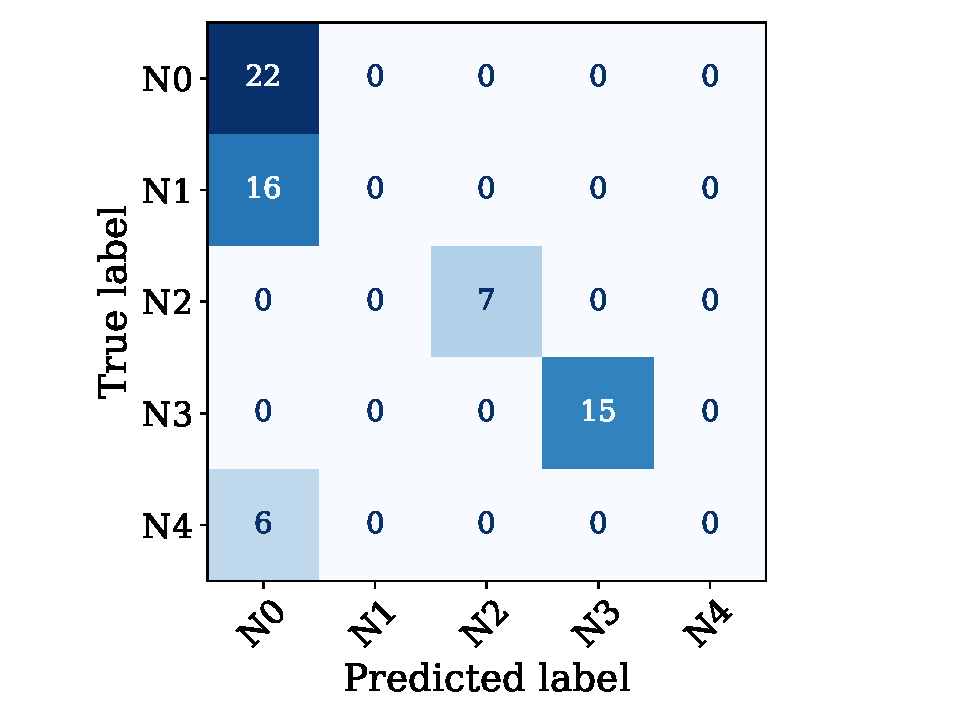
\includegraphics[width=0.50\columnwidth]{confusion_matrix1}}\hfill
	\subfloat[]{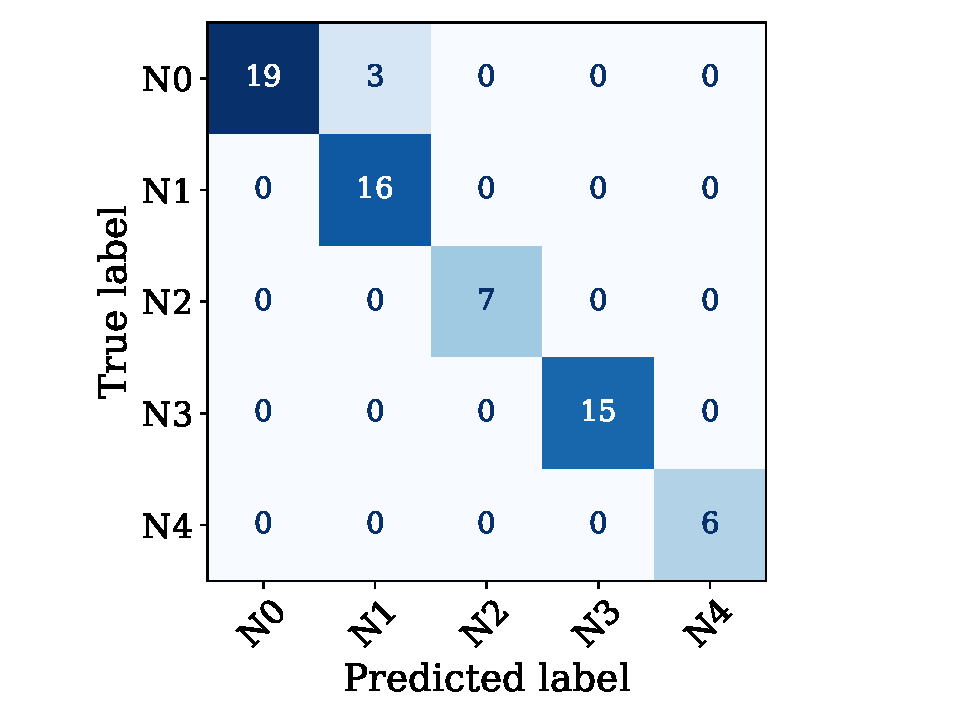
\includegraphics[width=0.50\columnwidth]{confusion_matrix2}}\hfill
	\subfloat[]{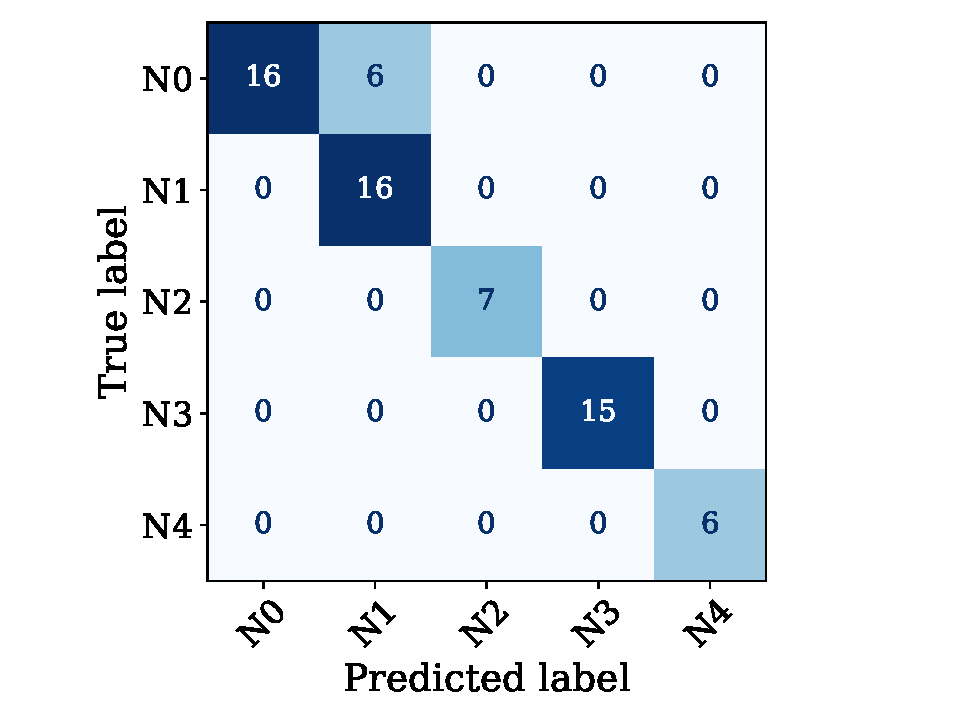
\includegraphics[width=0.50\columnwidth]{confusion_matrix3}}\hfill
	\subfloat[]{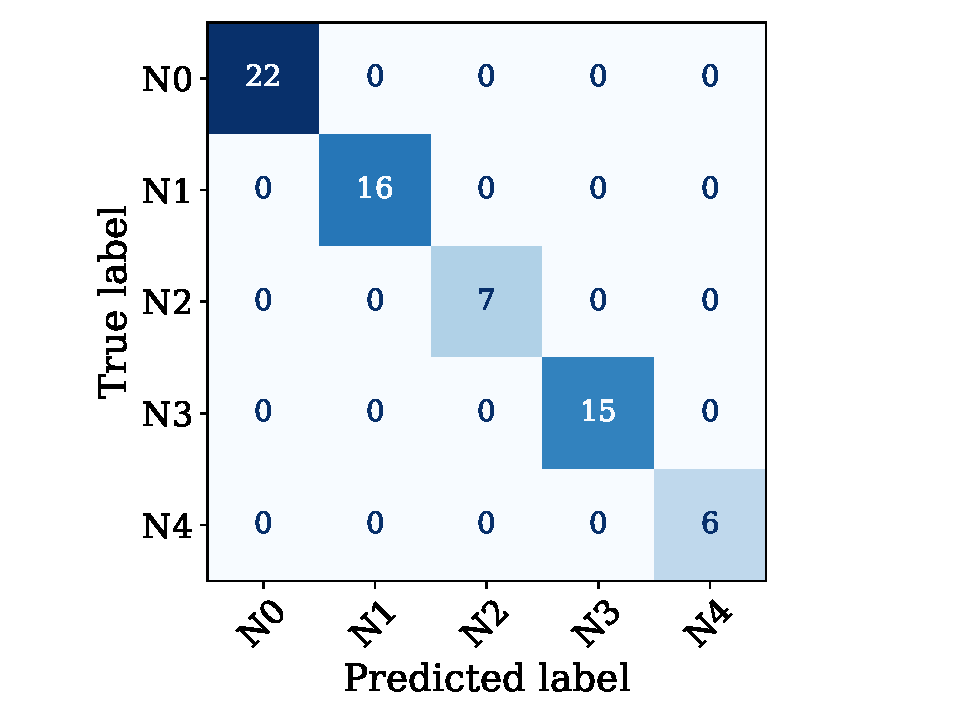
\includegraphics[width=0.50\columnwidth]{confusion_matrix4}}
	
	
	\caption{Fault diagnosis confusion matrix of four classifiers. (a) LeNet, (b) ResNet, (c) ConvNext, (d) AlexNet-SE.}
	\label{fig11}
\end{figure}	



\begin{enumerate}
	\item{The LeNet model performs the worst in terms of fault classification, with a large number of misclassifications in the N0, N1 and N4 category. Its overall accuracy is relatively low.}
	\item{Both the ResNet and ConvNeXt models show significant improvement over LeNet, with the ability to accurately classify the N1, N2, N3, and N4 categories. Although ResNet and ConvNext models show slight misclassifications for the N0 categories, their overall performance remains stable, achieving high accuracy.}
	\item{The AlexNet-SE performs the best, accurately classifying nearly all fault categories, demonstrating the model's outstanding performance and superior classification ability in this task.}
\end{enumerate}

In summary, while all four classifiers show some performance across different categories, the AlexNet-SE model stands out with its higher accuracy, making it the most exceptional model in this experiment. This experiment compares the performance of four different network architectures in fault diagnosis tasks, including AlexNet-SE, LeNet, ResNet, and ConvNext. Table IV analyzes the performance changes of different models after adding PINN.

\begin{enumerate}
	\item{Performance of PCNN combined with AlexNet-SE. The combination of Mel-GADF-PCNN and AlexNet-SE performs exceptionally well across all evaluation metrics, particularly achieving very high results in accuracy, precision, and \(F_1\) score. This outcome suggests that the integration of PCNN with Mel-GADF features, especially when combined with the AlexNet-SE model, demonstrates outstanding performance in fault diagnosis tasks, effectively capturing complex patterns and features in the data.}
	\item{Performance improvement after adding PINN. PINN+AlexNet-SE shows a significant performance improvement, especially excelling in accuracy, and precision. In contrast, the performance of other PINN combinations is noticeably inferior, particularly PINN+LeNet, which achieves only $72.24\%$ accuracy and $83.08\%$ precision. Although PINN+ResNet and PINN+ConvNext show some improvement, they still cannot compete with PINN+AlexNet-SE.}
\end{enumerate}

The experimental results show that, despite AlexNet-SE performing exceptionally well, the combination of PINN and AlexNet-SE further enhances the performance in fault diagnosis tasks, particularly with a significant improvement in $F_1$ score and \(G_{mean}\). This demonstrates that PINN can effectively augment the performance of AlexNet-SE. In contrast, while other PINN combinations show some improvement, they still fall short of reaching the performance level of PINN+AlexNet-SE. In conclusion, PINN+AlexNet-SE provides the optimal solution for fault diagnosis tasks, fully showcasing the immense potential of PINNs in enhancing the performance of traditional neural networks.


\section{Conclusion}
In this study, to address the challenges of limited fault data and low recognition accuracy in practical transformer fault diagnosis, we propose an improved PINN-based method. The approach enhances the feature extraction process and incorporates modifications to the baseline AlexNet architecture. A transformer voiceprint feature extraction strategy is adopted to effectively capture discriminative acoustic features, thereby improving the quality and representativeness of the training data. The extracted features are then utilized for fault classification using four PINN-based classifiers: LeNet, ResNet, ConvNeXt, and AlexNet-SE. To validate the effectiveness of the proposed method, comparative experiments were conducted using data before and after PCNN-based feature enhancement. The results demonstrate a significant improvement in classification performance across all classifiers, highlighting the compatibility and robustness of the proposed approach. This confirms the method’s ability to address the low classification accuracy issues prevalent in existing fault diagnosis models.

In future work, we aim to further optimize the proposed framework to improve recognition accuracy under more diverse and complex operating conditions, with the ultimate goal of enhancing the reliability and applicability of intelligent transformer faults diagnosis systems.


  \bibliographystyle{elsarticle-num-names} 
  \bibliography{references}

\end{document}

\endinput